\documentclass[11pt]{article}
\usepackage{graphicx, fancyhdr}
\usepackage{amsmath, amsfonts}
\usepackage{color, hyperref}
\usepackage{enumerate}
\usepackage{longtable}
\providecommand{\tightlist}{%
  \setlength{\itemsep}{0pt}\setlength{\parskip}{0pt}}
 
\newcommand{\blue}[1]{{\color{blue} #1}}

\setlength{\topmargin}{-.375 in}
\setlength{\textheight}{8.75 in}
\setlength{\textwidth}{6.5 in}
\setlength{\evensidemargin}{0 in}
\setlength{\oddsidemargin}{0 in}
\setlength{\parindent}{0 in}
\renewcommand{\headrulewidth}{0.4pt}
\renewcommand{\footrulewidth}{0.4pt}

\lhead{Stat 305} 
\chead{Competency Quiz 3} 
\rhead{Tuesday, April 9}
\lfoot{Spring 2019}
\cfoot{\thepage} 
\rfoot{} 

\def\Exp#1#2{\ensuremath{#1\times 10^{#2}}}
\def\Case#1#2#3#4{\left\{ \begin{tabular}{cc} #1 & #2 \phantom
{\Big|} \\ #3 & #4 \phantom{\Big|} \end{tabular} \right.}

\begin{document}
\pagestyle{fancy} 

Show \textbf{all} of your work on this assignment and answer each question fully in the given context. You have 20 minutes. Each problem is designed to take 10 minutes. All answers in a topic must be correct for any credit for that topic. You may attempt multiple topics. You may use a calculator on this competency quiz. \\

\begin{enumerate}
\def\labelenumi{\arabic{enumi}.}
\item
  \textbf{Competency Topic: Discrete Random Variables}

  Suppose that \(X\) is a discrete random variable with a geometric
  distribution with probability of success \(p\). That is, \(X\) has a
  probability function that is written as
  \[ f(x) = \begin{cases} (1-p)^{x-1} (p) & x = 1, 2, ... \\ 0 & o.w \end{cases} \]
  The mean and variance of a geometric random variable are based on the
  value of \(p\) so that \(E(X) = \frac{1}{p}\) and
  \(Var(X) = \frac{1-p}{p}\).

  \begin{enumerate}
  \def\labelenumii{\alph{enumii}.}
  \tightlist
  \item
    Find the probability that \(X \ge 2\) (hints: you do not need to do
    an infinite sum; the answer may include the term \(p\)).
    \vspace{4cm}
  \item
    For any \(x \ge 1\) and positive integer \(k\), find an expression
    for the ratio \(f(x + k)/f(x)\). \vspace{4cm}
  \item
    Suppose that a particular geometric random variable has mean \(10\).
    Find the variance.
  \end{enumerate}
\end{enumerate}

\newpage

\begin{enumerate}
\def\labelenumi{\arabic{enumi}.}
\setcounter{enumi}{1}
\item
  \textbf{Competency Topic: Continuous Random Variables}

  A gamma random variable depends on two parameters, a ``rate'' paramter
  \(k\) and a ``scale'' parameter \(\theta\). In the case where the
  shape parameter \(k\) is a positive integer, the probability density
  function can be written as:
  \[f(x) = \begin{cases} \dfrac{1}{(k-1)! \theta^k} x^{k-1} \exp\left(-\frac{x}{\theta}\right) & x \ge 0 \\ 0 & o.w. \end{cases}\]

  \begin{enumerate}
  \def\labelenumii{\alph{enumii}.}
  \tightlist
  \item
    Using the plot below, provide a rough sketch of the following pdfs:
  \end{enumerate}

  \begin{itemize}
  \item
    \begin{enumerate}
    \def\labelenumii{(\arabic{enumii})}
    \tightlist
    \item
      the pdf of a gamma random variable with \(k = 3\) and \(\theta=1\)
      and
    \end{enumerate}
  \item
    \begin{enumerate}
    \def\labelenumii{(\arabic{enumii})}
    \setcounter{enumii}{1}
    \tightlist
    \item
      the pdf of a gamma random variable with \(k = 1\) and \(\theta=1\)
    \end{enumerate}
  \end{itemize}

  (for the sketch, it is enough to find and connect the values of the
  pdf at \(x = 0, 1, 2, 3, 4\))
\end{enumerate}

\begin{center}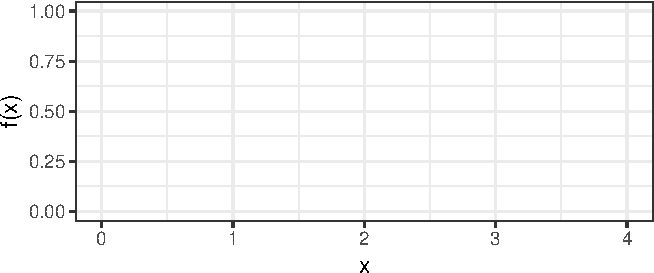
\includegraphics[width=.9\linewidth,height=.4\linewidth]{stat305-cq3_files/figure-latex/unnamed-chunk-2-1} \end{center}
   \vspace{3cm}

\begin{enumerate}
\def\labelenumi{\alph{enumi}.}
\setcounter{enumi}{1}
\tightlist
\item
  Based on your sketch, which of the two values of \(k\) will give the
  largest probability that \(X \le 1\)?
\end{enumerate}

\newpage

\begin{enumerate}
\def\labelenumi{\arabic{enumi}.}
\setcounter{enumi}{2}
\item
  \textbf{Competency Topic: Joint Distributions}

  Suppose that \(X\) follows a uniform distribution on \([0, 1]\) - that
  is, \(X\) has a density function such that \(f_X(x) = 1\) for
  \(0 \le x \le 1\) and \(f_X(x) = 0\) for any other value of \(x\).
  Also suppose that the joint distribution of \(X\) and a second random
  variable \(Y\) can be written as:
  \[ f_{XY}(x, y) = \begin{cases} \frac{4!}{y!(4-y)!} x^y (1-x)^{4-y} & 0 \le x \le 1, y = 0, 1, 2, 3, 4 \\ 0 & otherwise \end{cases} \]

  \begin{enumerate}
  \def\labelenumii{\alph{enumii}.}
  \tightlist
  \item
    Find the conditional probability density function of \(Y\) given
    \(X\), \(f_{Y|X}(y|x)\). \vspace{4cm}
  \item
    Find the probability that \(Y = 0\) given that \(X=0.1\).
    \vspace{3cm}
  \item
    Sketch the function \(f_{Y|X}(0|x)\) as a function of \(x\) (in
    otherwords, a sketch of how the probability that \(Y = 0\) changes
    as the value of \(X\) we are given changes)
  \end{enumerate}
\end{enumerate}

\begin{center}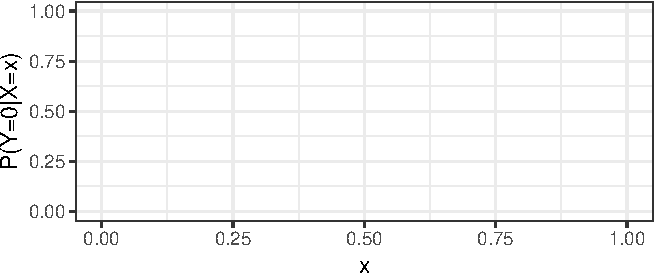
\includegraphics[width=.9\linewidth,height=.4\linewidth]{stat305-cq3_files/figure-latex/unnamed-chunk-3-1} \end{center}

\newpage

\begin{enumerate}
\def\labelenumi{\arabic{enumi}.}
\setcounter{enumi}{3}
\item
  \textbf{Competency Topic: Functions of Random Variables}

  Suppose that \(X\) and \(Y\) are independent discrete random variables
  where, for \(\lambda > 0\) and \(\alpha > 0\), the joint probability
  function can be written as:
  \[P(X=x, Y=y) = \begin{cases} \dfrac{\lambda^x}{x!} \exp\left(-\lambda\right) \dfrac{\alpha^y}{y!} \exp\left(-\alpha\right) & x = 0, 1, 2, ...; y = 0, 1, 2, ... \\ 0 & o.w. \end{cases}\]
  It can be show that \(E(X) = \lambda\) and \(Var(X) = \lambda\) and
  that \(E(Y) = \alpha\) and \(Var(Y) = \alpha\).

  Define \(U = X - Y\).

  \begin{enumerate}
  \def\labelenumii{\alph{enumii}.}
  \tightlist
  \item
    Find \(E(U)\) and \(Var(U)\). \vspace{3cm}
  \item
    Find the probability that \(U = 1\) (hints: consider the possible
    values of \(X\) and \(Y\) that could lead to \(U = 0\); also, your
    answer will include \(\lambda\) and \(\alpha\))
  \end{enumerate}
\end{enumerate}

\end{document}
